\documentclass[border=4pt]{standalone}
\usepackage{amsmath,amssymb}
\usepackage{tikz}
\usetikzlibrary{arrows.meta,shadows}
\begin{document}
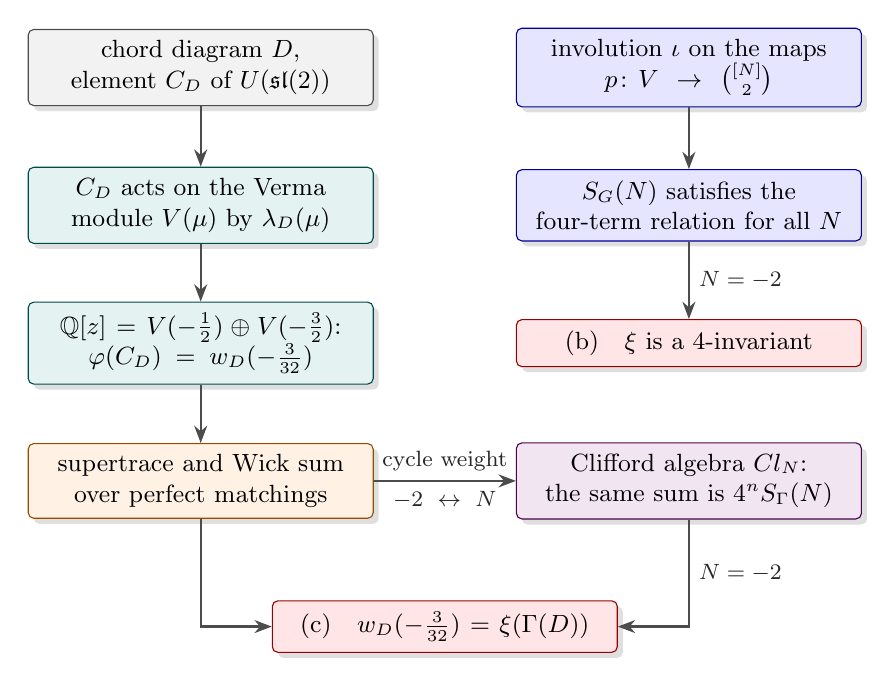
\begin{tikzpicture}[
  box/.style={draw=#1!60!black,fill=#1!10,rounded corners=2pt,align=center,
              font=\small,inner sep=4pt,text width=4.1cm,
              drop shadow={opacity=0.25,shadow xshift=2pt,shadow yshift=-2pt}},
  >={Stealth[length=2.2mm]}, arr/.style={->,thick,gray!60!black},
  note/.style={font=\footnotesize,gray!30!black,align=center}]
  \node[box=gray]   (cd) at (0,0)     {chord diagram $D$,\\ element $C_D$ of $U(\mathfrak{sl}(2))$};
  \node[box=teal]   (vm) at (0,-1.75) {$C_D$ acts on the Verma\\ module $V(\mu)$ by $\lambda_D(\mu)$};
  \node[box=teal]   (os) at (0,-3.5)  {$\mathbb{Q}[z]=V(-\tfrac12)\oplus V(-\tfrac32)$:\\ $\varphi(C_D)=w_D(-\tfrac{3}{32})$};
  \node[box=orange] (wk) at (0,-5.25) {supertrace and Wick sum\\ over perfect matchings};
  \node[box=violet] (cl) at (6.2,-5.25) {Clifford algebra $Cl_N$:\\ the same sum is $4^nS_{\Gamma}(N)$};
  \node[box=red]    (fc) at (3.1,-7.1) {(c)\quad $w_D(-\tfrac{3}{32})=\xi(\Gamma(D))$};
  \node[box=blue]   (inv) at (6.2,0)    {involution $\iota$ on the maps\\ $p\colon V\to\binom{[N]}{2}$};
  \node[box=blue]   (ft) at (6.2,-1.75) {$S_G(N)$ satisfies the\\ four-term relation for all $N$};
  \node[box=red]    (fb) at (6.2,-3.5)  {(b)\quad $\xi$ is a $4$-invariant};
  \draw[arr] (cd) -- (vm);
  \draw[arr] (vm) -- (os);
  \draw[arr] (os) -- (wk);
  \draw[arr] (wk) -- node[above,note]{cycle weight}node[below,note]{$-2\ \leftrightarrow\ N$} (cl);
  \draw[arr] (wk) |- (fc);
  \draw[arr] (cl) |- node[pos=0.25,right,note]{$N=-2$} (fc);
  \draw[arr] (inv) -- (ft);
  \draw[arr] (ft) -- node[right,note]{$N=-2$} (fb);
\end{tikzpicture}
\end{document}
